% % \begin{figure}
% % 	\centering
% 	\begin{minipage}{.5\textwidth}
% 		\centering
% 		\includegraphics[keepaspectratio]{Imagenes/exp1/biseccion_f.pdf}
% 		\captionof{figure}{A figure}
% 		\label{fig:test1}
% 	\end{minipage}%
% 	\begin{minipage}{.5\textwidth}
% 		\centering
% 		\includegraphics[keepaspectratio]{Imagenes/exp1/biseccion_f.pdf}
% 		\captionof{figure}{Another figure}
% 		\label{fig:test2}
% 	\end{minipage}
% \end{figure}

\begin{figure}[!h]
	\begin{center}
		  \includegraphics[keepaspectratio]{../Imagenes/exp1/biseccion_f.pdf}
		  \caption{Bisección\_f para $\alpha=4.0, \epsilon = 10^{-6}, criterio = 1\  con \ max\_iter=20$}
		  \label{fig:contra1}
	\end{center}
\end{figure}

~

\begin{figure}[!h]
	\begin{center}
		  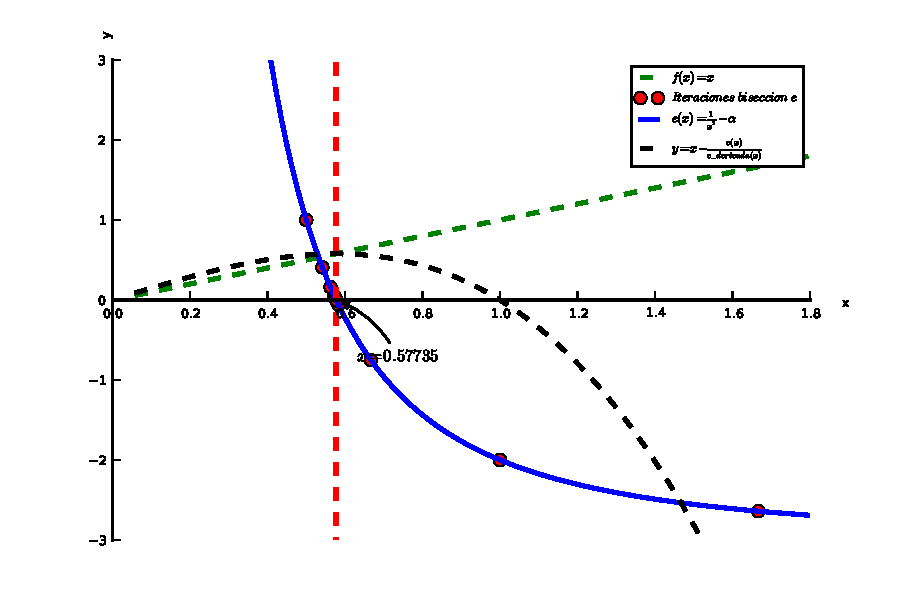
\includegraphics[keepaspectratio]{../Imagenes/exp1/biseccion_e.pdf}
		  \caption{Bisección\_e para $\alpha=6.0, \epsilon = 10^{-6}, criterio = 3$}
		  \label{fig:contra1}
	\end{center}
\end{figure}

Los resultados tanto para $biseccion\_f$ como para $biseccion\_e$ fueron los esperados. Los métodos convergen al resultado para cualquier valor de $\alpha$ (Fueron evaluados valores entre 0 y 10000 aproximadamente,
con bastante granularidad). Para realizar los gráficos fueron elegidos los valores de $\alpha$ 4.0 para $f$ y 6.0 para $e$ únicamente debido a que permiten utilizar una escala que nos deja apreciar los aspectos
relevantes del análisis. Los puntos rojos corresponden al valor de $x$ en cada iteración del método. Con el correr de las iteradas, los puntos van amontonándose alrededor de la raíz teórica de la función.

Un aspecto llamativo de los resultados obtenidos en esta etapa es el hecho de que 
a medida que los valores de $\alpha$ crecen, bisección\_e requiere de una mayor cantidad de iteraciones (en comparación con $f$) para obtener un valor cercano a la raíz de la función. Por ejemplo,
tomando 40 iteraciones en cada experimento y variando el valor de alfa, obtuvimos que: 

Para $\alpha = 0.1$, $f(x\_40) \approx 1*10^{-13}$ y $e(x\_40) \approx 1*10^{-13}$. 

Para $\alpha = 7.0$ : 
$f(x\_40) \approx 1*10^{-11}$ y $e(x\_40) \approx 1*10^{-10}$. 

Y ya para $\alpha = 10000.0$: $f(x\_40) \approx 1*10^{-5}$ y $e(x\_40) \approx 0.01$

Notemos que estamos utilizando el criterio (3) para analizar la calidad de la solución obtenida.

Por lo general biseccion\_e se comprta peor que biseccion\_f (Terminar de pensar por qué)


